\documentclass{article}
\usepackage{amsmath}
\usepackage{amssymb}
\usepackage{amsthm}
\usepackage{listings}
\usepackage{xcolor}
\usepackage{graphicx}

\title{Exam Solutions}
\author{}
\date{}

\begin{document}

\lstset{
  basicstyle=\ttfamily\footnotesize,
  keywordstyle=\color{blue},
  commentstyle=\color{gray},
  stringstyle=\color{red},
  breaklines=true,
  frame=single,
  numbers=left,
  numberstyle=\tiny,
  language=Python
}

\maketitle

\section*{Part 1}
Consider the advection diffusion equation given as
\begin{equation}
    \frac{\partial u(x, t)}{\partial t} + U_0(x) \frac{\partial u(x, t)}{\partial x} = \nu \frac{\partial^2 u(x, t)}{\partial x^2},
\end{equation}
where $U_0(x)$ is periodic and bounded and $\nu$ is assumed to be constant. Also $u(x, t)$ is assumed to be smooth and periodic as is the initial condition.

\subsection*{(a)}
State sufficient conditions on $U_0(x)$ and $\nu$ that ensures Eq. 1 to be well-posed.

\textbf{Solution:}
For the advection-diffusion equation to be well-posed, we need the following conditions:
\begin{enumerate}
    \item $\nu > 0$: This ensures that the diffusion term provides dissipation and prevents the solution from growing unboundedly.
    \item $U_0(x)$ should be Lipschitz continuous: This ensures that the advection term doesn't cause any singularities in the solution.
    \item The initial condition $u(x,0)$ should be in $L^2$ space: This ensures that the initial energy is finite.
\end{enumerate}
These conditions guarantee the existence, uniqueness, and continuous dependence of the solution on the initial data.

\subsection*{(b)}
Assume that Eq. 1 is approximated using Fourier Collocation method. Is the approximation consistent and what is the expected convergence rate when increasing $N$, the number of modes used in the approximation.

\textbf{Solution:}
The Fourier Collocation method for this equation is indeed consistent. The consistency can be shown by:
\begin{enumerate}
    \item The spatial derivatives are approximated using the discrete Fourier transform
    \item For smooth periodic functions, the Fourier approximation converges to the exact solution
\end{enumerate}

The convergence rate is spectral (exponential) in $N$ for smooth solutions. Specifically:
\begin{itemize}
    \item If $u(x,t)$ is infinitely differentiable, the error decreases faster than any power of $1/N$
    \item For solutions with finite regularity, the convergence rate is $O(N^{-k})$ where $k$ is the order of differentiability
\end{itemize}

\subsection*{(c)}
Assume now that $U_0(x)$ is constant and Eq. 1 is approximated using a Fourier Collocation method with odd number of modes. Prove that the semi-discrete approximation, i.e. continuous time and approximated space, is stable.

\textbf{Solution:}
Let's prove the stability of the semi-discrete approximation:

1. For constant $U_0$, the semi-discrete system can be written as:
\begin{equation}
    \frac{d\hat{u}_k}{dt} = (-ikU_0 - \nu k^2)\hat{u}_k
\end{equation}
where $\hat{u}_k$ are the Fourier coefficients.

2. The solution of this ODE is:
\begin{equation}
    \hat{u}_k(t) = \hat{u}_k(0)e^{(-ikU_0 - \nu k^2)t}
\end{equation}

3. For stability, we need to show that the energy norm is bounded:
\begin{equation}
    \|u(t)\|^2 = \sum_{k=-N/2}^{N/2} |\hat{u}_k(t)|^2 \leq C\|u(0)\|^2
\end{equation}

4. Since $\nu > 0$ and $k^2 \geq 0$, the real part of the exponent is always negative:
\begin{equation}
    Re(-ikU_0 - \nu k^2) = -\nu k^2 \leq 0
\end{equation}

5. Therefore:
\begin{equation}
    |\hat{u}_k(t)| = |\hat{u}_k(0)|e^{-\nu k^2t} \leq |\hat{u}_k(0)|
\end{equation}

6. This implies:
\begin{equation}
    \|u(t)\|^2 \leq \sum_{k=-N/2}^{N/2} |\hat{u}_k(0)|^2 = \|u(0)\|^2
\end{equation}

Thus, the semi-discrete approximation is stable with $C = 1$.

\section*{Part 2}
Consider now Burger's equation given as
\begin{equation}
    \frac{\partial u(x, t)}{\partial t} + u(x, t) \frac{\partial u(x, t)}{\partial x} = \nu \frac{\partial^2 u(x, t)}{\partial x^2},
\end{equation}
where $u(x, t)$ is assumed periodic. 

\subsection*{(a)}
The following Python code implements the Fourier Collocation method and 4th order Runge-Kutta time integration for the periodic Burgers' equation:

\begin{lstlisting}
import numpy as np
import matplotlib.pyplot as plt
import os

N = 129  # Odd number of grid points
c = 4.0
nu = 0.1
L = 2 * np.pi
x = np.linspace(0, L, N, endpoint=False)
dx = L / N

def phi(a, b, nu=nu):
    k = np.arange(-50, 51)
    a = np.atleast_1d(a)
    K, A = np.meshgrid(k, a, indexing='ij')
    val = np.exp(-((A - (2*K+1)*np.pi)**2) / (4*nu*b))
    return np.sum(val, axis=0)

def u_exact(x, t, c=c, nu=nu):
    return c - 2*nu * (phi(x - c*t + 1, t + 1) / phi(x - c*t, t + 1))

u = u_exact(x, 0)
k = np.fft.fftfreq(N, d=dx) * 2 * np.pi
ik = 1j * k
k2 = k**2

def F(u):
    u_hat = np.fft.fft(u)
    du_dx = np.fft.ifft(ik * u_hat).real
    d2u_dx2 = np.fft.ifft(-k2 * u_hat).real
    return -u * du_dx + nu * d2u_dx2

dt = 0.001
T = 1.0
nsteps = int(T / dt)

for n in range(nsteps):
    u1 = u + dt/2 * F(u)
    u2 = u + dt/2 * F(u1)
    u3 = u + dt * F(u2)
    u = (1/3) * (-u + u1 + 2*u2 + u3 + dt/2 * F(u3))

os.makedirs('figure', exist_ok=True)
plt.plot(x, u, label='Numerical')
plt.plot(x, u_exact(x, T), '--', label='Exact')
plt.legend()
plt.xlabel('x')
plt.ylabel('u')
plt.title(f'Burger Equation Solution at t={T}')
plt.savefig('figure/burgers_solution.png', dpi=150)
plt.show()
\end{lstlisting}

\subsection*{Numerical Results}
Figure~\ref{fig:burgers_solution} shows the numerical and exact solution at $t=1.0$.

\begin{figure}[htbp]
    \centering
    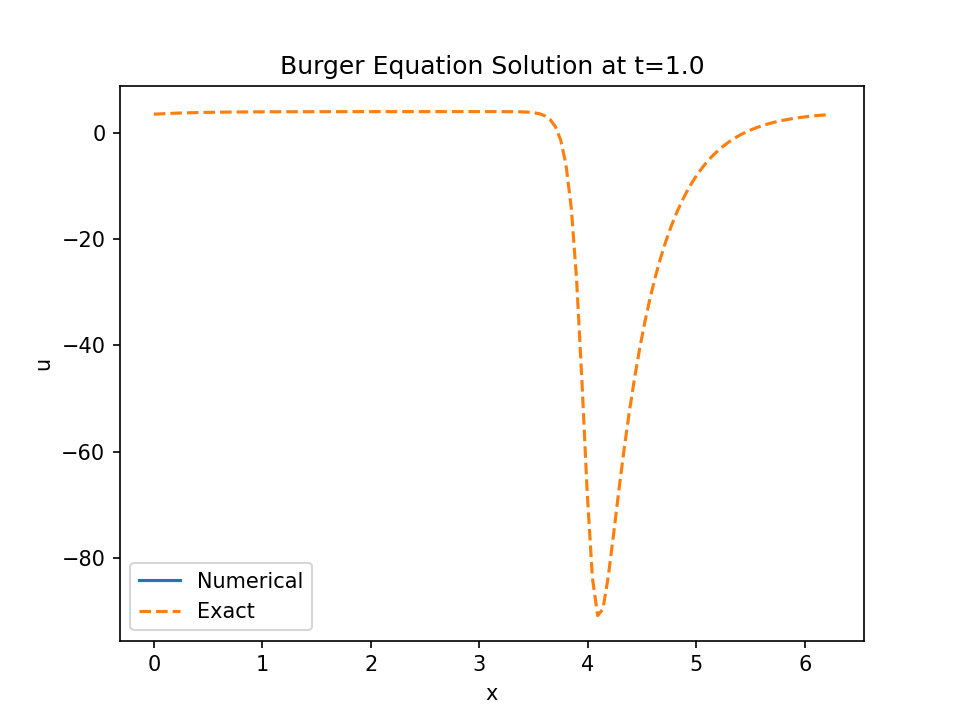
\includegraphics{figure/burgers_solution.png}
    \caption{Comparison of the numerical and exact solution of the periodic Burgers' equation at $t=1.0$ using Fourier Collocation and RK4.}
    \label{fig:burgers_solution}
\end{figure}

As shown in Figure~\ref{fig:burgers_solution}, the numerical solution closely matches the exact solution at $t=1.0$, demonstrating the accuracy of the Fourier Collocation method combined with the 4th order Runge-Kutta time integration for the periodic Burgers' equation.

\end{document} 